%\documentclass[twocolumn]{article}
\documentclass[11pt]{article}
\usepackage[top= 1.7cm,
bottom = 2.0cm,
left   = 2.2cm,
right  = 2.2cm]{geometry}
\usepackage[latin1]{inputenc}
\usepackage[T1]{fontenc}
\usepackage{tikz}
\usepackage{textcomp}
\usepackage{ae,aecompl,amsmath,amsbsy,amssymb,eurosym}
\usepackage{graphicx}
\usepackage{longtable}
\usepackage{appendix}
\usepackage{float}
\usepackage{bm}
%\usepackage{natbib}
\usepackage{placeins}
\usepackage[hang, flushmargin, bottom]{footmisc}
\usepackage{graphics}
\usepackage{multicol}
\usepackage{adjustbox}
\usepackage{cite}
\usepackage{enumerate}
\usepackage[normalem]{ulem} 
\usepackage{color}
\usepackage{setspace}
\usepackage{caption}
\usepackage{ifthen}
\usepackage{multirow}
%\usepackage[font={bf}]{caption}
\usepackage{pdflscape}
\usepackage{enumerate}
\usepackage{enumitem}
\usepackage{listings}
\usepackage{longtable}
\usepackage[all]{xy}
\usepackage{pdfpages}
\xyoption{frame}
\usepackage[latin1]{inputenc}
%\usepackage[TABTOPCAP]{subfigure}
\usepackage{subcaption}
\usepackage{amsthm,amsmath,natbib}
\usepackage[hyperfootnotes=false]{hyperref}
\hypersetup{
 colorlinks=true,
 linkcolor=red,
 citecolor=blue,
 linktoc=page,
 urlcolor=blue}
\usepackage[all]{hypcap}
\usepackage{fancyhdr}
\pagenumbering{arabic}
\numberwithin{equation}{section}
\usepackage{parskip}
\setlength{\parskip}{0.3cm plus1mm minus1mm}
\linespread{1.10}
\usepackage{pdfpages}

\renewcommand{\figurename}{Fig.}

\begin{document}
\vspace{-6cm}
\title{{\bf {\Large Propuesta para Mejorar las Medidas de Valor Agregado de Escuelas en Per\'u}}}
\author{Claudia Allende SC}
\vspace{-6cm}
\date{\today}
\maketitle

\section*{Resumen}

\begin{itemize}

\item Las medidas de {\it Value Added} (Valor Agregado) son ampliamente usadas en sistemas educativos, ya que ofrecen una medida precisa de la contribuci\'on de las escuelas al aprendizaje, limpia de factores que son externos a las decisiones que toman las escuelas.
\item En coordinaci\'on con el Minsiterio de Educaci\'on y otras entidades estatales, el Ministerio de Econom\'ia y Finanzas, lider\'o la recopilaci\'on de los datos necesarios para una primera estimaci\'on de las medidades de valor agregado de escuelas en Per\'u. Estos datos ya se est\'an empleando para la toma de decisiones y la evaluaci\'on de pol\'iticas p\'ublicas.
\item Esta propuesta consiste en mejorar las medidas de valor agregado usando informaci\'on de RENIEC que permite vincular de manera exacta la informaci\'on  de los padres de famila con la informaci\'on del alumno.
\item Para evitar infringir los acuerdos de confidencialidad de datos, los investigadores desarrollar\'an un proceso que permita generar las medidas sin tener acceso directo a los datos sensibles.

\end{itemize}	

\section{Antecedentes}

\begin{itemize}
\item {\bf \textquestiondown Qu\'e son las Medidas de Valor Agregado?}. Las medidas de {\it Value Added} (valor agregado) se usan para estimar o cuantificar qu\'e porci\'on de los resultados acad\'emicos de los alumnos pueden ser atribuidos a la escuela (o profesor). En otras palabras, se busca aislar la contribuci\'on de la escuela al aprendizaje del alumno de otros factores que afectan el aprendizaje (como los antecedentes socioecon\'omicos de los alumnos o lo aprendido por los alumnos en instituciones a las que asistieron previamente). El objetivo es obtener mediciones que reflejen la verdadera calidad de una escuela (el valor que agrega, al menos en t\'erminos de resultados acad\'emicos en pruebas estandarizadas) y no estos otros factores que, en general, son externos a las decisiones que toman las escuelas y no deber\'ian ser considerados a la hora de ser evaluados. Para m\'as detalles sobre la estrategia emp\'irica ver el ap\'endice I.


\item {\bf Su uso en la pr\'actica}. En varios distritos escolares en el mundo estas medidas de calculan sistem\'aticamente y se utilizan para evaluar escuelas y tomar decisiones sobre retenci\'on y compensaci\'on de los profesores. En serie de estudios recientes por Chetty, Friedman y Rockoff (2014a, 2014b) proveen una rica discusi\'on que defiende el uso de estas medidas en t\'erminos t\'ecnicos. Adem\'as, muestran que estas medidas de calidad (en el caso de calcularse al nivel individual del profesor) est\'an altamente correlacionadas con mejores resultados futuros\footnote{Usando datos para m\'as de un mill\'on de ni\~nos, encuentran que los estudiantes asignados a los maestros de mayor valor agregado son m\'as propensos a asistir a la universidad, ganar salarios m\'as altos, y son menos propensos a tener hijos como adolescentes.}, validando el uso de este tipo de medidas. Por su lado, Deming (2014) muestra que las estimaciones de VAM son similares a los resultados usando asignaci\'on aleatoria, lo que se conoce como el {\it golden standard} en t\'erminos de evaluaci\'on de impacto.\footnote{En su estudio no puede rechazar la hip\'otesis de que los impactos de las escuelas son estimaciones insesgadas del avances reales de los alumnos medidos a trav\'es de asignaci\'on aleatoria.}


\item {\bf Primera Versi\'on de las Medidas de Valor Agregado.} El Ministerio de Econom\'ia y Finanzas, a trav\'es de la Direcci\'on General de Presupuesto P\'ublico, lider\'o la recopilaci\'on de informaci\'on logrando vincular informaci\'on del registro de matricula del MINEDU (SIAGIE) con las siguientes fuentes de informaci\'on:
\begin{itemize}
    \item Resultados de la Evaluaci\'on Censal de Estudiantes (ECE)
    \item Censo de Poblaci\'on y Vivienda (CPV)
    \item Registro del Certificado del Nacido Vivo (CNV)
    \item Padr\'on General de Hogares del SISFOH (PGH)
\end{itemize}

Esta mediciones ya se est\'an empleando para el dise\~{n}o de pol\'iticas p\'ublicas. (Ver Ap\'endice)

 Para esta medici\'on no se consigui\'o datos que permitan vincular de manera exacta la informaci\'on del alumno con la informaci\'on de los padres de familia por lo que se tuvo que recurrir a t\'ecnicas probabil\'isticas de vinculaci\'on. Si bien las mediciones son \'utiles para la toma de decisiones, estas se podr\'ian mejorar sustancialmente con datos que permitan una vinculaci\'on exacta del estudiante con los padres de familia.

\end{itemize}
\section{Motivaci\'on} 


\begin{itemize}


\item {\bf} La Direcci\'on General de Presupuesto P\'ublico tiene entre sus funciones programar, dirigir, coordinar, controlar y evaluar la gesti\'on del proceso presupuestario\footnote{Seg\'un el art\'iculo 4 de la Ley General del Sistema Nacional de Presupuesto (Ley N$^\circ$28411)}. Asimismo, dentro de las funciones de la Direcci\'on de Calidad del Gasto P\'ublico, de la Direcci\'on General de Presupuesto P\'ublico, se encuenta el realizar estudios prospectivos del gasto del sector p\'ublico en el marco de los objetivos de pol\'tica del pa\'is y sus correspondientes planes nacionales y territoriales, en coordinaci\'on con las unidades org\'anicas competentes del Ministerio.
\item\ En l\'inea con estas funciones, las medidas de valor agregado de las escuelas aportan informaci\'on valiosa para la toma de decisiones presupuestales y de evaluaci\'on del gasto p\'ublico del sector educaci\'on. 
\item Adem\'as, el ejercicio sienta un precedente adicional para impulsar institucionalidad para generar estas medidas en el futuro, con acuerdos que perduren en el tiempo que permitan desarrollar mejores y m\'as completas bases de datos, de forma de poder incluirlas en el dise\~no y evaluaci\'on de nuevas pol\'iticas p\'ublicas.



\end{itemize}

\section{Implementaci\'on}


\begin{itemize}

\item {\bf}  Para calcular las medidas de valor agregado es necesario contar con un vector de caracter\'isticas del alumno (ver la ecuaci\'on 4.1 en el ap\'endice I, vector $X_{it}$). De estas caracter\'isticas, un subconjunto de ellas son caracter\'isticas de los padres de familia que se requieren vincular al alumno.

\item {\bf} En el ejercicio de medici\'on anterior el Ministerio de Econom\'ia y Finanzas logr\'o recopilar todos los datos sociodemogr\'aficos. Adem\'as recientemente el MEF logr\'o obtener acceso a informaci\'on de RENIEC que permite vincular a los estudiantes con sus respectivos padres de familia. 

\item {\bf} En concreto, es necesario:
\begin{itemize}
    \item Conocer el esquema de las tablas que intervienen en el ejercicio con el mayor detalle posible: nombre de las columnas, claves primarias, tipo de datos, tipo de relaci\'on con las otras tablas y estad\'isticas descriptivas sencillas de las tablas. 
    \item A partir de esta informaci\'on se desarrollar\'a un c\'odigo que tendr\'an como resultado las medidas de valor agregado a nivel de escuela para las evaluaciones de matematicas y razonamiento verbal de la ECE.
\end{itemize}

\item En la medici\'on anterior, las bases cruzadas fueron entregadas a los investigadores libres de identificadores individuales y bajo los par\'ametros de un de acuerdo confindecialidad que cumple con los est\'andares del Ministerio de Econom\'ia, el Ministerio de Educaci\'on y los lineamientos del {\it Research Integrity Assurance} (Aseguramiento de la Integridad de la Investigaci\'on) de la Universidad de Princeton.

\item {\bf Timeline de este proyecto}

\begin{itemize}

\item {\bf Acuerdos:} Redacci\'on de propuesta de para acuerdo de trabajo y protocolo de manejo de datos {\bf [Uno o dos d\'ias]}.

\item {\bf Esquemas:} Una vez aceptada la propuesta, se enviar\'an a los investigadores la informaci\'on detallada de las tablas que intervienen en el proyecto {\bf [Una semana]}.

\item {\bf Desarrollo de C\'odigo:} Los investigadores desarrollar\'an  el c\'odigo para generar el valor agregado con los datos  {\bf [Una o dos semanas]}.

\item {\bf Pruebas} El c\'odigo generar\'a reportes parciales durante el proceso para asegurar que los c\'alculos sean correctos. En caso se presenten errores se coordinar\'a para ajustar el c\'odigo.  {\bf [Una semana]}. 

\item {\bf Base Final}: Se le enviar\'an a los investigadores las bases a nivel de escuela de acuerdo a los protocolos de seguridad de datos acordados entre el MEF, MINEDU y los investigadores.

\end{itemize}	

\end{itemize}

\newpage

\section*{Ap\'endice}
  

\subsection*{\bf Estrategia emp\'irica}  
Se busca limpiar los resultados acad\'emicos del alumno de factores relacionados al entorno del que este proviene, ya que estos pueden afectar considerablemente su rendimiento acad\'emico. Para estimar los Modelos de Value Added (MVA), su utilizan resultados de pruebas estandarizadas en distintos momentos del tiempo, combinados con otra informaci\'on sobre los estudiantes. La forma general es:

\begin{equation}\label{eq:qualityOLS}
Test\_Score_{ijt}= X_{it} \beta + \omega_{ijt}, \hspace{0.3cm} \omega_{ijt}=\mu_j+\theta_{jt}+\epsilon_{ijt}
\end{equation}

Donde $Test\_Score_{ijt}$ es el puntaje de la prueba estandarizada (ECE en ese caso) en determinada asignatura (Lenguaje o Matem\'aticas) para el estudiante $i$, en la escuela $j$ en el a\~no $t$, $X_{it}$ es un vector de caracter\'isticas a nivel del estudiante, y $\omega_{ijt}$ es el residuo, que se compone de un efecto fijo a nivel de escuela $\mu_j$, que es nuestro par\'ametro de inter\'es\footnote{Existen distintas formas de calcular este par\'ametro: calculando el residuo promedio a nivel de escuela (es decir, {\it random effects} o mediante estimaci\'on directa (es decir, {\it fixed effects})} y que interpretaremos como el valor agregado promedio de la escuela
. Dependiendo de los supuestos que se hagan y la forma de estimar este modelo, se puede interpetar $\theta_{jt}$ de distintas formas: 

\begin{itemize} 

\item VA fijo en el tiempo: se asume que $\theta_{jt}+\epsilon_{ijt}$ son errores i.i.d. y que el VA de la escuela no cambia en el tiempo (razonable si se cuentan con datos de pocos a\~nos).

\item VA din\'amico: se asume que el valor agregado de las escuelas puede cambiar en el tiempo, y que el Valor Agregado es el efecto total $\omega_{ijt} + \theta_{jt}$ a nivel de escuela.

\end{itemize}



\subsection*{\bf Ejemplo para Chile.} 

\vspace{0.7cm}
\begin{table}[h!]
\caption{Estimaciones de Valor Agregado}
\begin{center}
 \scriptsize{
\begin{tabular}{lccccc} \hline
& \multicolumn{2}{c}{Model 1 (Reduced)} & &  \multicolumn{2}{c}{Model 2 (Expanded)}  \\ \cline{2-3} \cline{5-6}
    & Coef. & StdErr      & & Coef. &  StdErr    \\ \hline
Constant	   	 &  0.082	 & ( 0.002)	  &  	 & -1.699	 & ( 0.058)	\\
Mother More High School	   	 &  0.316	 & ( 0.003)	   	 & &  0.213	 & ( 0.003)	\\
Mother High School   	   	 &  0.201	 & ( 0.002)	   	 & &  0.190	 & ( 0.002)	\\
Father More High School	   	 & - 	 & - 	   	 & &  0.213	 & ( 0.003)	\\
Father High School	   	 & - 	 & - 	   	 & &  0.101	 & ( 0.002)	\\ \hline
Poor	   	 & -0.122	 & ( 0.002)	   	 & & -0.093	 & ( 0.002)	\\
Male	   	 & -0.035	 & ( 0.002)	   	 & & -0.049	 & ( 0.002)	\\
Married	   	 & - 	 & - 	   	 & &  0.003	 & ( 0.002)	\\
Birth Weight (mg)	   	 & - 	 & - 	   	 & &  0.001	 & ( 0.000)	\\
Birth Weight$^2$, (mg)  	   	 & - 	 & - 	   	 &  & -0.000	 & ( 0.000)	\\
Birth Gestation	(wk)   	 & - 	 & - 	   	 &&  0.012	 & ( 0.001)	\\
Birth Gestation$^2$	(wk)   	 & - 	 & - 	   	 & & -0.000	 & ( 0.000)	\\
Birth Length (cm)	   	 & - 	 & - 	   	&   &  0.031	 & ( 0.002)	\\
Birth Length$^2$ (cm)	   	 & - 	 & - 	   	 & & -0.000	 & ( 0.000)	\\
Single Birth	   	 & - 	 & - 	   	 & & -0.026	 & ( 0.027)	\\
Number of siblings	   	 & - 	 & - 	   	&  & -0.029	 & ( 0.001)	\\
Twin	   	 & - 	 & - 	   & 	 & -0.083	 & ( 0.027)	\\
Birth Father Age	   	 & - 	 & - 	   	&  &  0.002	 & ( 0.000)	\\
Birth Mother Age	   	 & - 	 & - 	   	&  &  0.004	 & ( 0.000)	\\
\hline
$R^2$	  	                    &    0.30  	&	 	  	& &  0.32	 	&	 	      \\
N obs	  	 	                &   1,380,255	&        &    & 1,380,255	&               \\
\hline
\end{tabular}
} 
\end{center}
\end{table}

\newpage
\subsection*{\bf Uso del Valor Agregado en el MINEDU} 

Uno de los usos del valor agregado fue determinar si existe correlaci\'on entre la probabilidad de acceder a un cr\'edito del programa {\bf Reactiva Per\'u} y el valor agregado.


\begin{figure}[!htb]
    \begin{minipage}[b]{0.99\textwidth}
        \begin{center}
            \caption{Correlaci\'on entre Valor Agregado y Probabilidad de Acceder a Reactiva}
            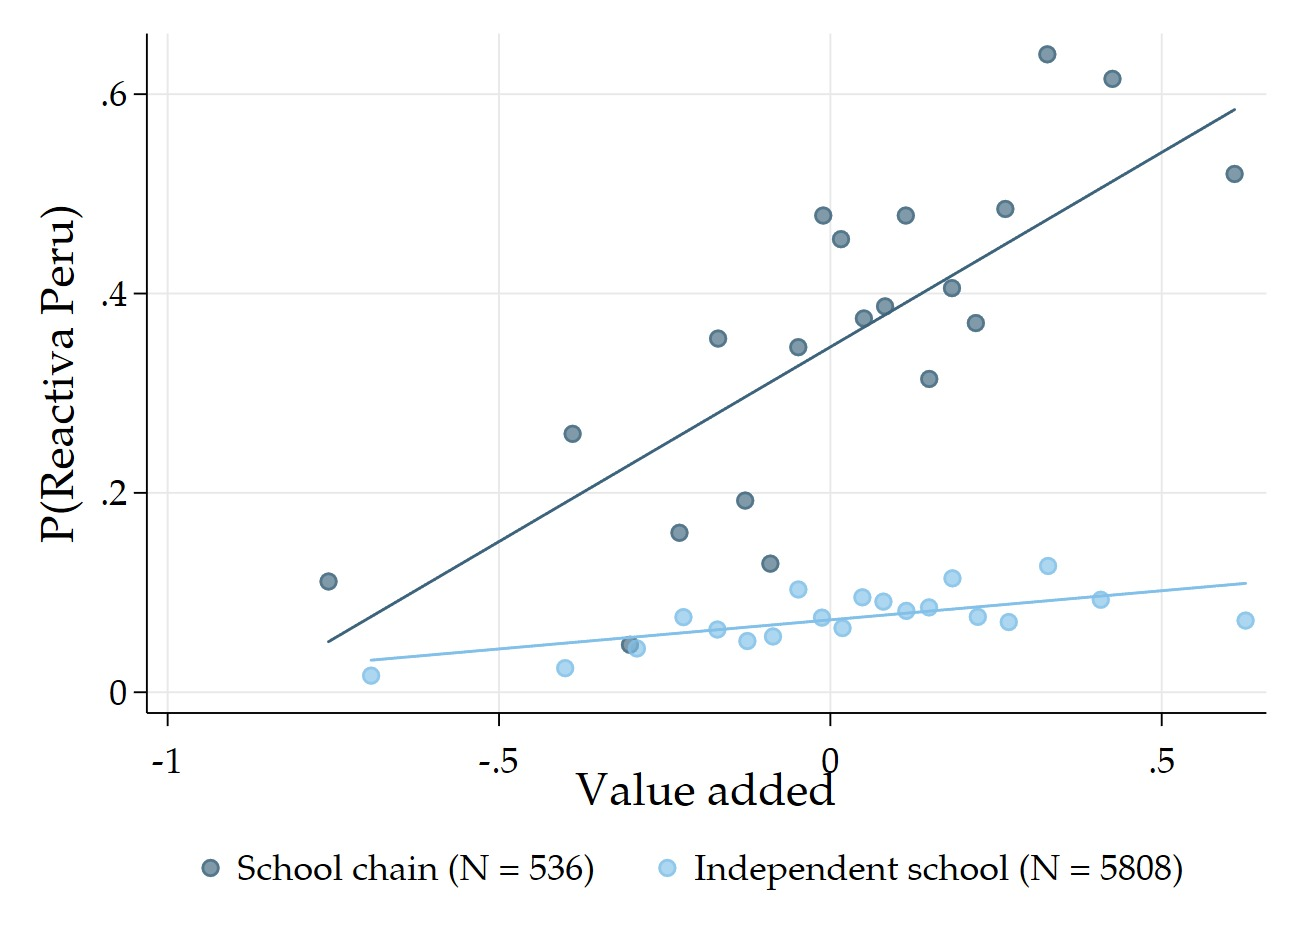
\includegraphics[scale=0.29]{figures/ReactivaVA.jpeg}
            
        \end{center}

    \end{minipage}
\end{figure}
Se observa una correlaci\'on positiva entre la probabilidad de acceder al cr\'edito y el valor agregado de la escuela, la cual es m\'as acentuada en colegios que pertenecen a una cadena educativa. 

Otro uso de las medidas de valor agregado fue evaluar el potencial impacto en la calidad de la ense\~{n}anza en los alumnos que estaban migrando de colegios privados a colegios p\'ublicos debido a la pandemia.

\begin{figure}[!htb]
\caption{Valor Agregado del Colegio de Origen vs. Colegio de Destino por sector Socioecon\'omico \newline Lima}
    \begin{minipage}[b]{0.99\textwidth}
        \minipage{0.3\textwidth}
            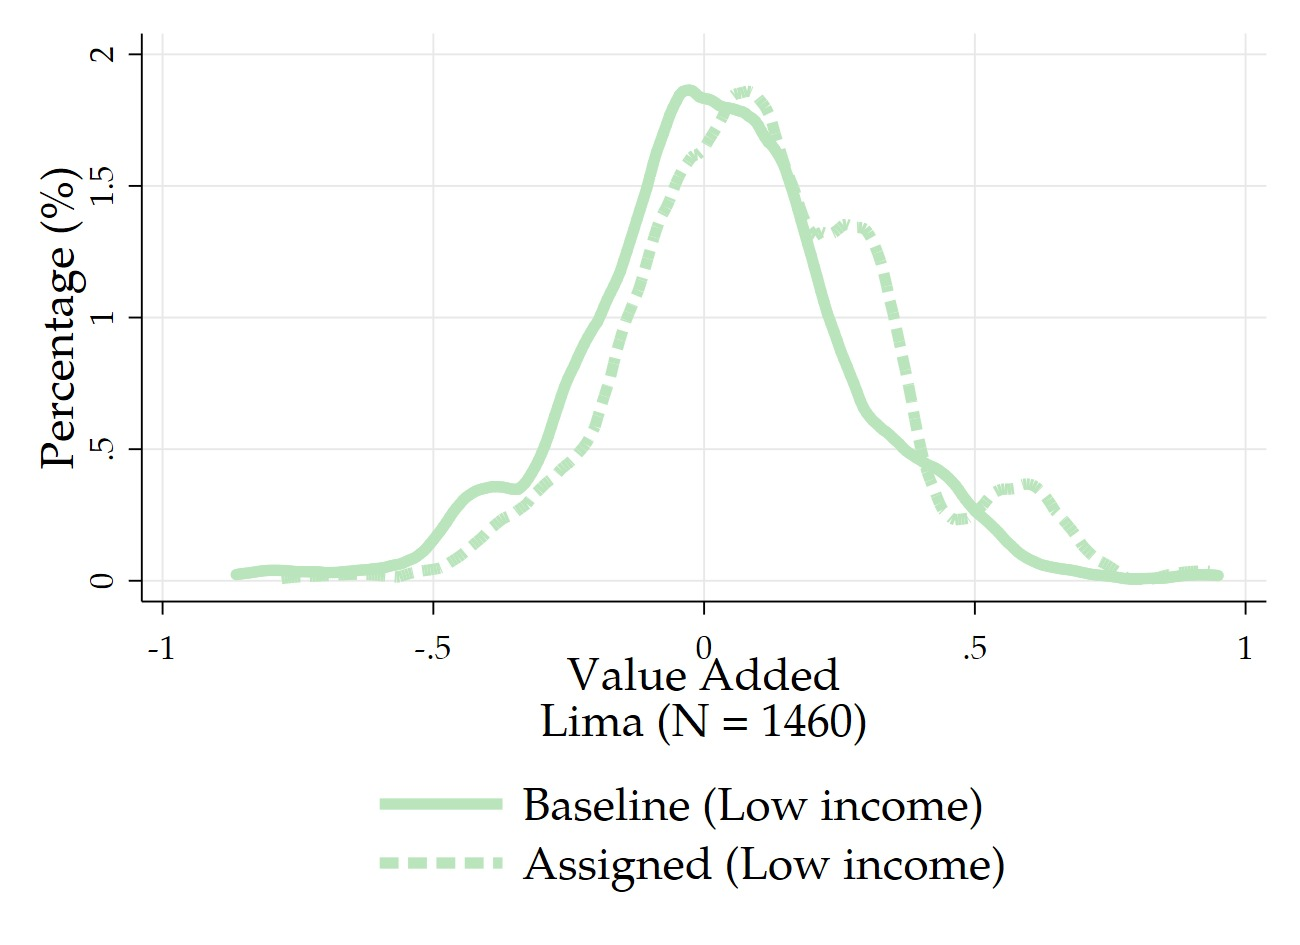
\includegraphics[width=\linewidth]{figures/LimaLI.jpeg}
            \label{fig:LimaLI}
        \endminipage
        \hfill
        \minipage{0.3\textwidth}
            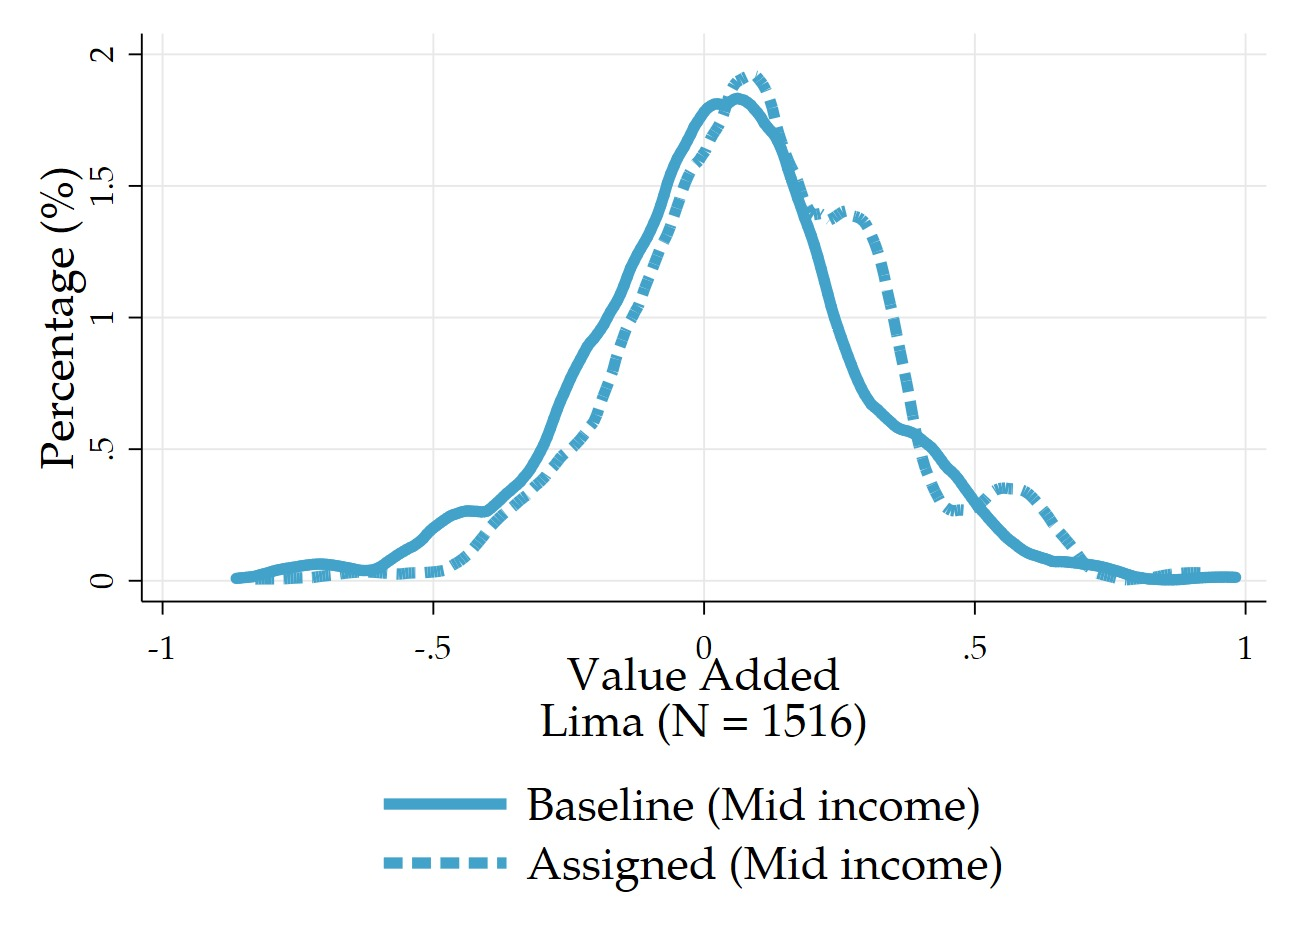
\includegraphics[width=\linewidth]{figures/LimaMI.jpeg}
            \label{fig:LimaMI}
        \endminipage
        \hfill
        \minipage{0.3\textwidth}
            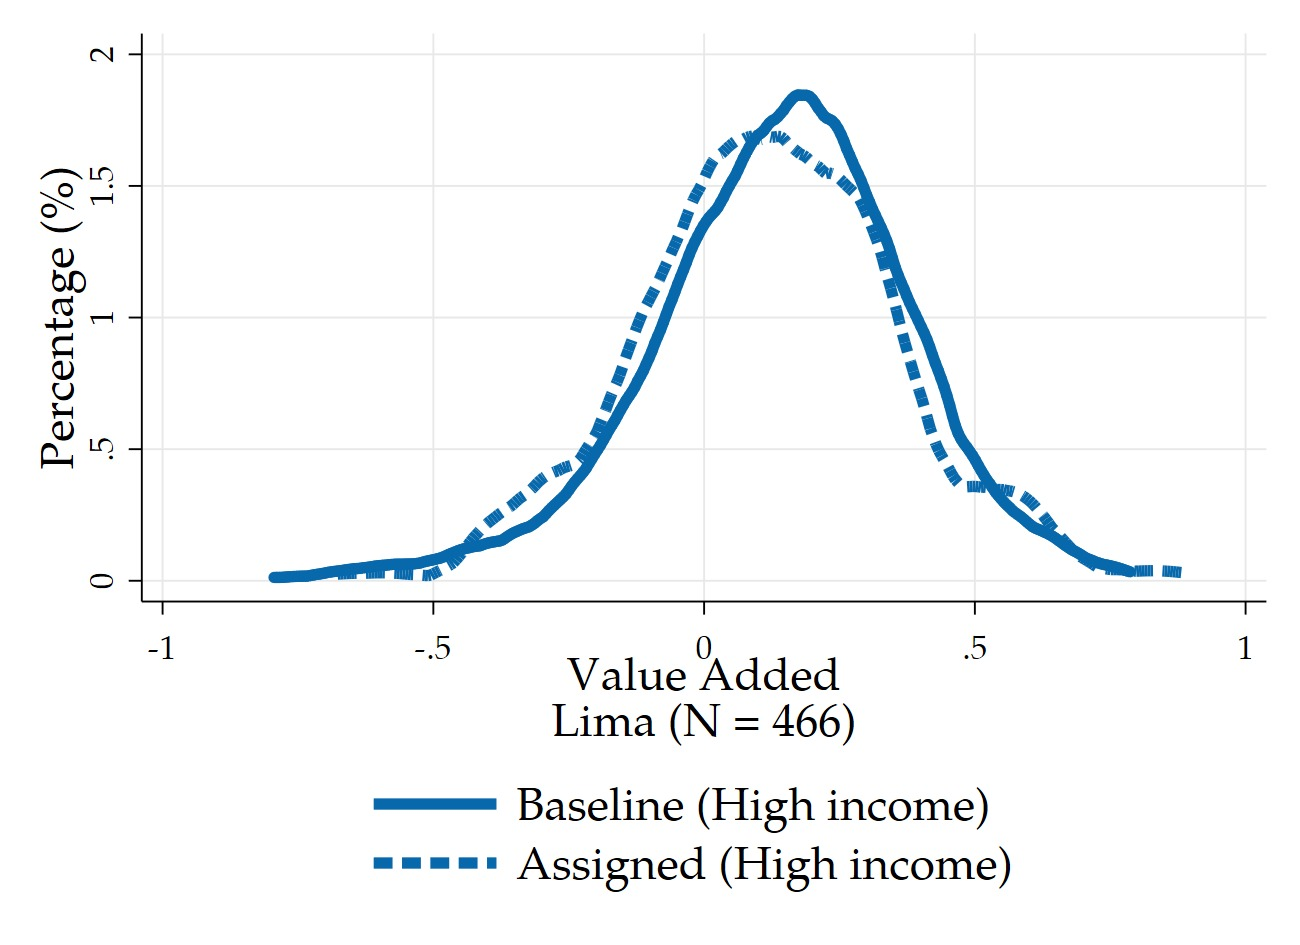
\includegraphics[width=\linewidth]{figures/LimaHI.jpeg}
            \label{fig:LimaHI}
        \endminipage
    \end{minipage}
\end{figure}

Para el caso de Lima, se observa una mejora para ciertos segmentos de la distribuci\'on en alumnos de sectores socioecon\'omicos bajo y medio. Para el caso de alumnos del sector socioecon\'omico alto, s\'i se observa una ligera disminuci\'on en el valor agregado del colegio de destino.  

\begin{figure}[!htb]
\caption{Valor Agregado del Colegio de Origen vs. Colegio de Destino por sector Socioecon\'omico \newline No Lima}
    \begin{minipage}[b]{0.99\textwidth}
        \minipage{0.3\textwidth}
            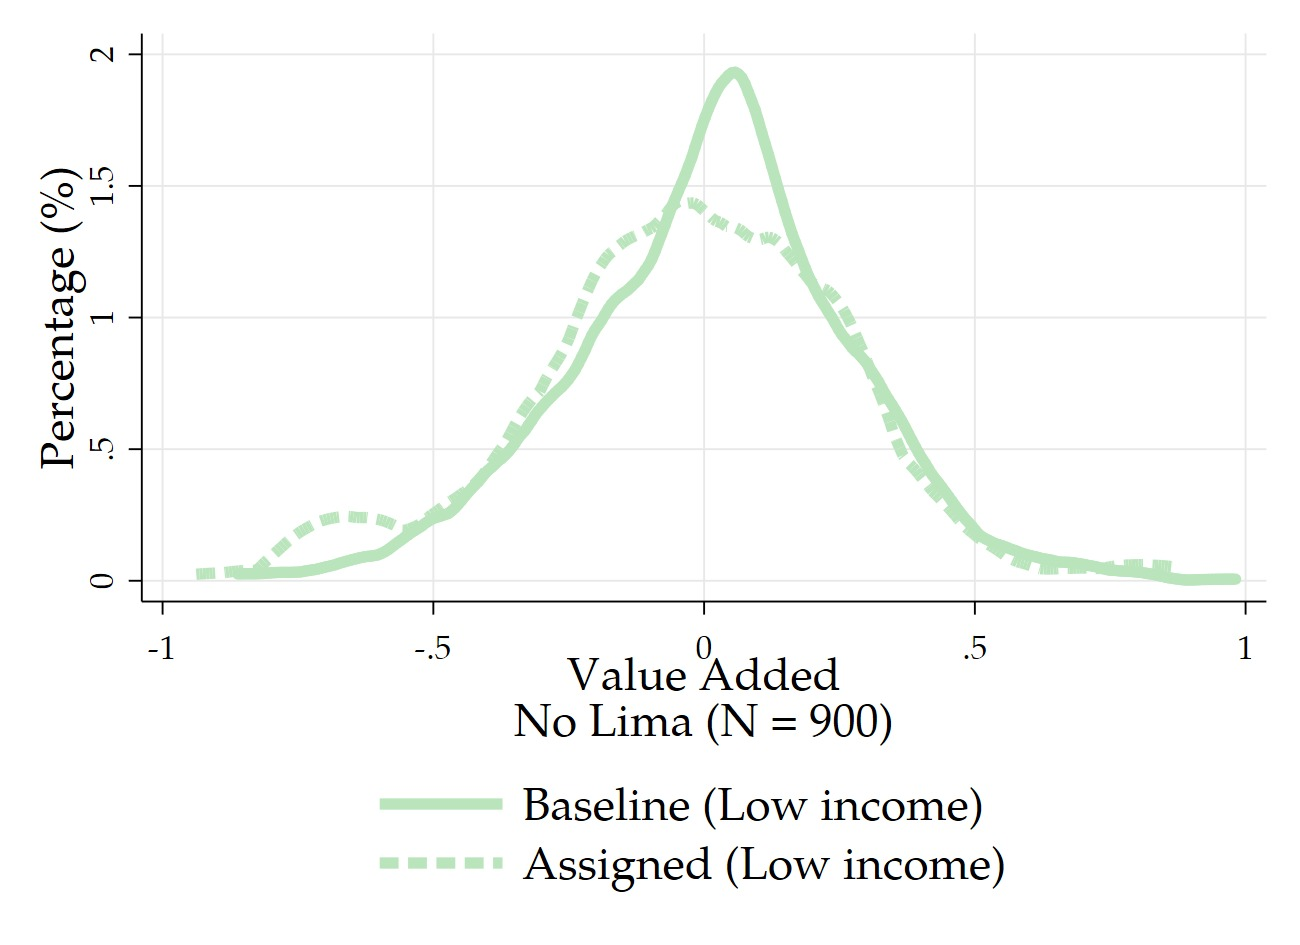
\includegraphics[width=\linewidth]{figures/NoLimaLI.jpeg}
            \label{fig:LimaLI}
        \endminipage
        \hfill
        \minipage{0.3\textwidth}
            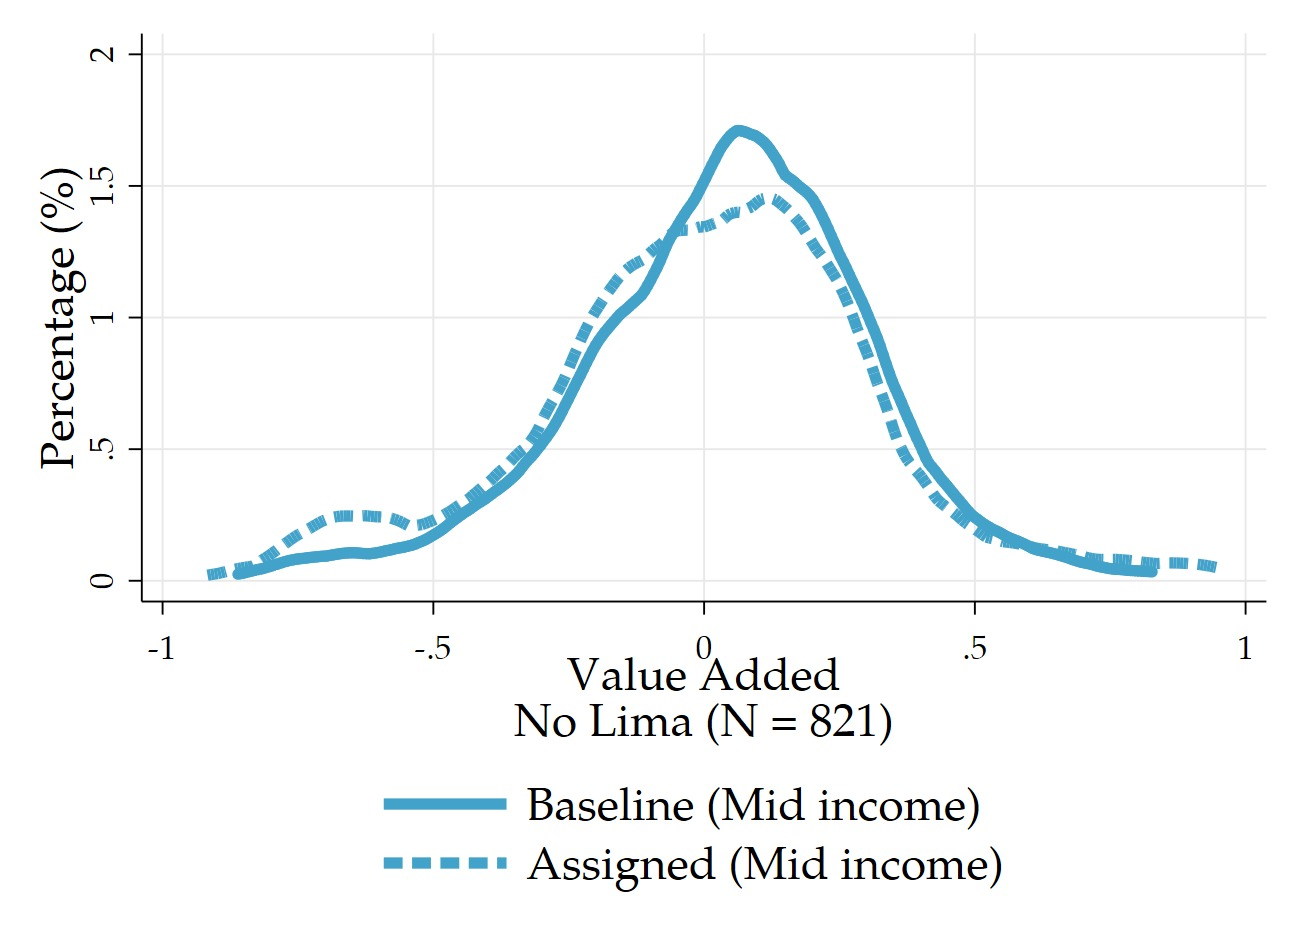
\includegraphics[width=\linewidth]{figures/NoLimaMI.jpeg}
            \label{fig:LimaMI}
        \endminipage
        \hfill
        \minipage{0.3\textwidth}
            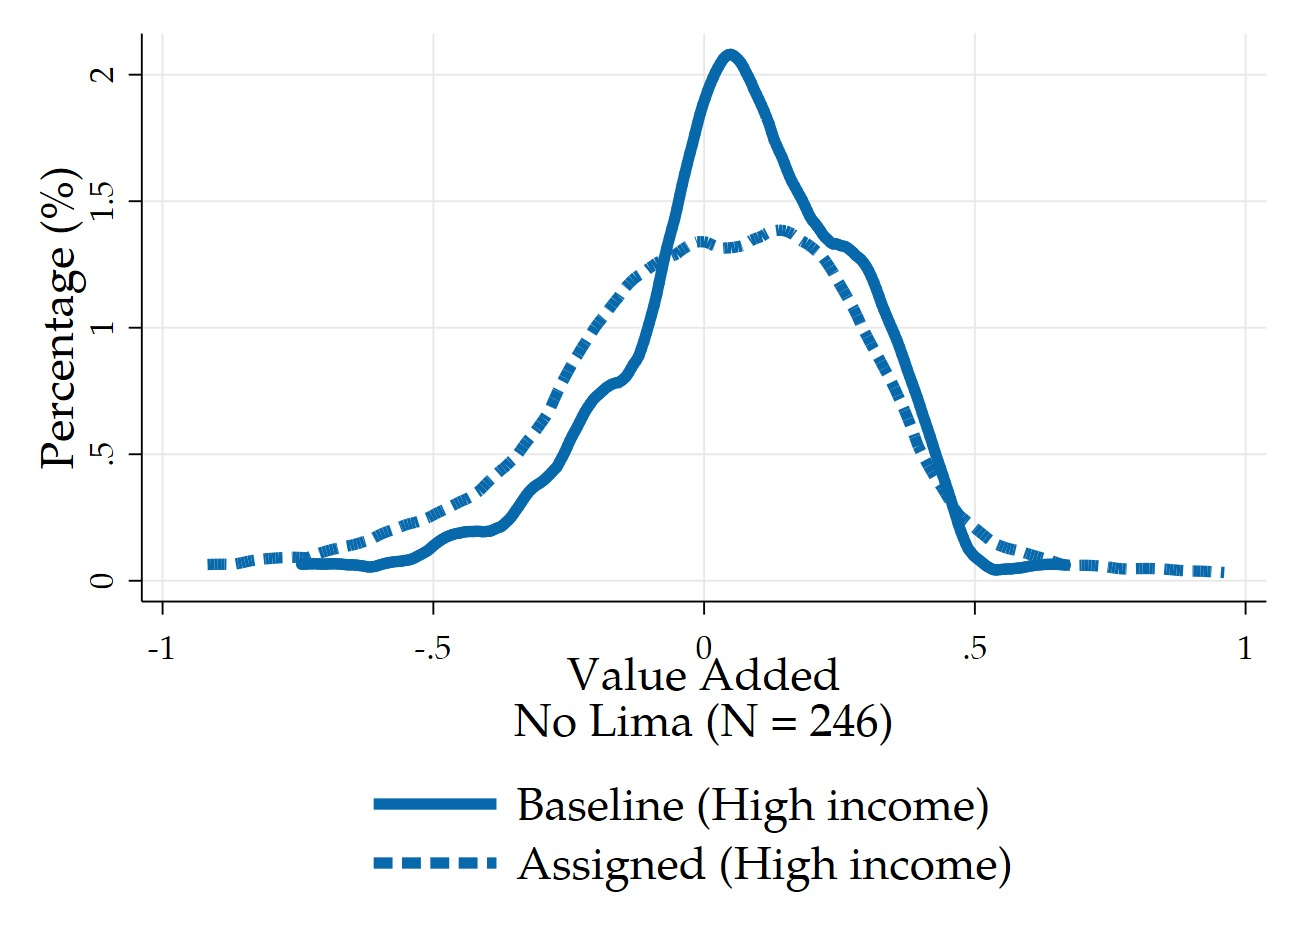
\includegraphics[width=\linewidth]{figures/NoLimaHI.jpeg}
            \label{fig:LimaHI}
        \endminipage
    \end{minipage}
\end{figure}
Para el caso de alumnos que viven fuera de Lima, se observa un incremento en la variabilidad del valor agregado de la escuela de destino para todos los sectores socioecon\'omicos y una ligera disminuci\'on, la cual es m\'as acentuada en el sector sociecon\'omico alto.  
% The vector of characteristics used in my empirical estimation is unusually large relative to the literature and includes detailed information on the student's family background. The estimated value of $q_{jt}$ is the school fixed effect and is the component of the average test score in the school that is not explained by the individual characteristics of the students. This will capture the school inputs such as teacher quality, infrastructure and any other school specific characteristic that raises the average test score. To the extent that the demographic composition of the schools' students matter for test scores, these effects will also be included in the school fixed effect quality measure.\footnote{\citeasnoun{altonji2010estimating} considers a wide array of assumptions regarding the role of peer composition in determining test scores.}

% Important assumptions are made in the estimation of school quality. I do not model peer effects directly and I assume that $v_{ijt}$ is orthogonal to $q_{jt}$ which precludes selection on unobservable characteristics. These assumptions are restrictive but provide a parsimonious model that can produce counterfactual test score distributions in a tractable way. In practice, estimation will be carried out with a  large  vector of family observable characteristics to limit the extent of selection driving the estimates. Moreover, the growth in aggregate test scores documented in \hyperref[figure:DD_Scores]{Figure \ref*{figure:testscore_evolution}} is not likely to be driven by selection effects or peer effects. This suggests that these assumptions will not be critical for the results in the paper and are discussed further in \hyperref[sec:results]{Secton \ref*{sec:results}}.



% School quality is estimated by OLS according to  \hyperref[eq:qualityOLS]{Equation \ref*{eq:qualityOLS}}.
% The school quality is the  school and year fixed effect in a regression of  students test scores that controls for a large vector of student characteristics including household income, detailed parental educational levels, mothers' math and language college entrance exam scores, demographic composition of the family, and early childhood health indicators.

%  \hyperref[table:VA_RegressionResults]{Table \ref*{table:VA_RegressionResults}}  presents the results which include school and year fixed effects. The top panel shows the role of parents education and the mothers college entrance exam results in math and language. Both parents' education have significant and relatively large coefficients. Students whose mother took the college entrance exam also did significantly better, adding almost $0.3\sigma$ to the students' test scores. Mothers who did better on the college entrance exam also had children who did better on 4th grade evaluations. A mother who scored one standard deviation above the mean test score in language had children who scored $0.3\sigma$ better. Interestingly, mothers' performance on math tests are much less important in magnitude than language test scores by a factor of four or five.

% Health at birth has been shown to be a important predictor of later life outcomes\footnote{See \citeasnoun{behrman2004returns},\citeasnoun{currie2011human}, and \citeasnoun{almond_currie_2011_AER} for examples.}.  \citeasnoun{Bharadwaj_Loken_Neilson_2013_AER} show that health outcomes are systematically correlated with academic outcomes in the case of Chile. The results shows that birth weight, birth length and weeks of gestation are all significantly related to test scores, even after controlling for school and year fixed effects as well as many other demographic characteristics. %Household income per capita percentile rank and a indicator for being below the 40th percentile are also significant predictors of test scores as is having an internet connection and a computer at home.
% %
% %\begin{table}[h]
% %\begin{center}
% %\begin{minipage}[h]{0.8\textwidth}
% %\caption{School Quality Estimation Regression}\label{table:VA_RegressionResults}
% %[UPDATE VA Regs]
% %%\input{Tables/VA_RegressionsTables}
% %\footnotetext{\mynoindent Note: This table presents regression results for estimates of test scores on a large vector of individual student level characteristics. School quality is estimated as the school and year fixed effect and have not been  presented in this table.   }
% %\end{minipage}
% %\end{center}
% %\end{table}

% The resulting school and time fixed effect estimates for school quality are too numerous to present in a table. I summarize two main results that stem from this analysis. The first is
% that, consistent with the results from the literature on school quality in Chile summarized in \citeasnoun{drago_paredes2011}, voucher schools have higher quality than public schools on average and private non-voucher schools have much higher quality than either. An additional result that is less emphasized in the literature is that school quality as measured in this application is very heterogeneous within types of schools as can be seen in Figure \ref{figure:Distribution_VA_DEP}. I find that this significant heterogeneity is smaller within local markets but still significant.%\footnote{A regression of estimated quality in 2007 on year and school type fixed effects has an $R^2$ of 0.30 while adding market fixed effects  }
% %Finally market structure as measured by the number, type and quality of nearby schools are all found to be significantly correlated with school quality.

% \begin{figure}[h]\centering
% \noindent\begin{minipage}[h]{0.8\textwidth}\centering
% \caption{Distribution of Estimated School Quality by School Type in 2011}\label{figure:Distribution_VA_DEP}
% \bigskip

% \input{Figures/Dist_VA}
% \footnotetext{\hspace{-0.25in} Note: This figure shows the distribution of quality estimated  for schools in 2011 using \ref{eq:qualityOLS}. Regression coefficients are presented in \autoref{table:VA_RegressionResults}.  }
% \end{minipage}
% \end{figure}

% The second result is that school quality rose both in the aggregate and within public and voucher schools but did not change at all in the non voucher private sector which did not participate in the SEP policy. Public schools improved evenly across the distribution while lower performing voucher schools improved the most. Table \ref{table:ChangeDistribution_VA} and Figure \ref{figure:ChangeDistribution_VA_DEP} present the growth in school quality by type of school across the distribution of achievement. Public schools improved their student weighted average quality by $0.16\sigma$ with larger improvements at higher quality part of the distribution. Voucher schools increased their quality by $0.12 \sigma$ on average with the largest changes coming from the bottom of the quality distribution.

% \begin{figure}[h]\centering
% \noindent\begin{minipage}[h]{0.99\textwidth}\centering
% \caption{Changes in the Distribution of School Quality by Type}\label{figure:ChangeDistribution_VA_DEP}
% \bigskip


% \input{Figures/ChangeDist_VA_Bars}
% \footnotetext{\hspace{-0.25in} Note: This figure shows the change in the distribution at the percentiles 10,25,50,75, and 90 of quality estimated  for schools averaging over 2005-2007 and comparing to the average of 2009-2011.  }
% \end{minipage}
% \end{figure}

% One natural check is to look at the relationship between estimated school quality and the schools inputs which from theory and other empirical evidence we think affect the quality of the school.  \autoref{table:VA_TeacherScore} plots the nonparametric relationship between a voucher school's estimated quality and the average college entrance exam math test scores of the teachers at the school.\footnote{This measure has been shown in other work to be related to teacher quality measured in several ways \cite{alvarado_neilson_2013}.}
% The positive correlation between inputs and our estimated quality measure is reassuring. We might also think that if a school is indeed better at raising test scores, it would be expected to raise its prices. In \autoref{table:VA_Price} we see a positive relationship between school quality and prices charged by voucher schools, again confirming our expectations regarding the estimated quality measure.








\end{document}